% !BIB program = biber 
\documentclass{article}

%% Encoding
\usepackage[T1]{fontenc}
\usepackage[utf8]{inputenc}

%% Fonts
% Math fonts (fourier) with utopia (erewhon) text fonts
\usepackage{fourier, erewhon}
\usepackage{algorithm}
\usepackage[noend]{algpseudocode}

%% Setup
% This package contains logos
\usepackage[autoload]{adn}

\setlogos[
\textbf{MO433 --- Intro. to Unsupervised Machine Learning}\\%[5pt]
\uppercase{Instituto de Computação --- UNICAMP}\\%[-7pt]
]%
{IC3D}%
{UNICAMP}

%% Transform section references
\makeatletter
\renewcommand*{\p@section}{\S\,}
\renewcommand*{\p@subsection}{\S\,}
\makeatother

%% Shorthands
\usepackage{xspace}
\makeatletter
\DeclareRobustCommand\onedot{\futurelet\@let@token\@onedot}
\def\@onedot{\ifx\@let@token.\else.\null\fi\xspace}

\def\eg{e.g\onedot} \def\Eg{E.g\onedot}
\def\ie{i.e\onedot} \def\Ie{I.e\onedot}
\def\cf{cf\onedot} \def\Cf{Cf\onedot}
\def\etc{etc\onedot} \def\vs{vs\onedot}
\def\wrt{w.r.t\onedot} \def\dof{d.o.f\onedot}
\def\etal{et al\onedot}
\makeatother

%%%
% Other packages start here (see the examples below)
%%
\usepackage{caption}

%% Figues
\usepackage{graphicx}
\graphicspath{{./images/}}

%% References
% Use this section to embed your bibliography
% Instead of having a separate file, just place the bibtex entries here
\usepackage{filecontents}% create files
\begin{filecontents}{\jobname.bib}
  @article{zhang2018,
  author={Jing Zhang and Tong Zhang and Yuchao Dai and Mehrtash Harandi and Richard I. Hartley},
  title={Deep Unsupervised Saliency Detection: {A} Multiple Noisy Labeling Perspective},
  journal={CoRR},
  volume={abs/1803.10910},
  year={2018},
  url={http://arxiv.org/abs/1803.10910},
  archivePrefix={arXiv},
  eprint={1803.10910}
  }
  @article{symonyan2014,
  author={Karen Simonyan and Andrea Vedaldi and Andrew Zisserman},
  title={Deep Inside Convolutional Networks: Visualising Image Classification Models and Saliency Maps},
  journal={CoRR},
  volume={abs/1312.6034},
  year={2014},
  url={https://arxiv.org/pdf/1312.6034.pdf},
  archivePrefix={arXiv},
  eprint={1312.6034}
  }
  @article{zhang2014,
  author={Ali Borji and Ming{-}Ming Cheng and Huaizu Jiang and Jia Li},
  title={Salient Object Detection: {A} Survey},
  journal={CoRR},
  volume={abs/1411.5878},
  year={2014},
  url={http://arxiv.org/abs/1411.5878},
  archivePrefix={arXiv},
  eprint={1411.5878},
  }
  @inproceedings{zhang2017,
  author={D. {Zhang} and J. {Han} and Y. {Zhang}},
  booktitle={2017 IEEE International Conference on Computer Vision (ICCV)}, 
  title={Supervision by Fusion: Towards Unsupervised Learning of Deep Salient Object Detector}, 
  year={2017},
  volume={},
  number={},
  pages={4068-4076}
  }
  @article{wang2017,
    author="Wang, Jingdong and Jiang, Huaizu and Yuan, Zejian and Cheng, Ming-Ming and Hu, Xiaowei and Zheng, Nanning",
    title="Salient Object Detection: A Discriminative Regional Feature Integration Approach",
    journal="International Journal of Computer Vision",
    year="2017",
    volume="123",
    number="2",
    pages="251--268",
    issn="1573-1405",
    doi="10.1007/s11263-016-0977-3"
  }
\end{filecontents}
% Include bibliography file
\usepackage[
backend=biber, 
style=ieee, 
natbib=true,
]{biblatex}
\addbibresource{\jobname.bib}

%% Math
\usepackage{amsmath}

%% Enumerate
\usepackage{enumitem}

\begin{document}

% Put the topic of the assignment here
\title{Final Project Proposal \\
\large Deep Unsupervised Saliency Detection}
% Put your name here 
\author{
Jo\~ao Victor da Silva Guerra,
Leonardo Alves de Melo,
and Marcos Felipe de Menezes Mota
\thanks{117410, 156188 and 211893. j117410@dac.unicamp.br, leonardo.alves.melo.1995@gmail.com, and marcos.mota@ic.unicamp.br}
}

\maketitle

Saliency detection targets visually interesting regions in images that can attract human visual attention, which generates a namely saliency map that identifies pixel's unique features. These saliency maps aims at simplifying and/or changing the image into a more meaningful representation to analyze \cite{zhang2018, symonyan2014}. In computer vision, salient object detection is commonly a process consist of two stages: (1) detect the most salient object; (2) segment the accurate object region \cite{zhang2014}. In recent years, with the powerful learning capabilities of deep neural networks, convolutional models have been employed to address the task of salient object detection.

Deep learning saliency maps were introduced in \cite{symonyan2014}, which applied visualisation techniques to compute images, saliency maps being one of them. Building upon the capabilities of convolutional neural networks (CNN), these deep supervised saliency detection methods achieved state-of-the-art performance with greater performance compared to unsupervised methods \cite{zhang2018}. However, such supervised methods depends on large-scale manual supervision as pixel-level human annotations, which is highly time-consuming, labor-intensive and could hinder the generalization ability of the models \cite{zhang2018, zhang2014}. In the literature, "Supervision by Fusion" (SBF; \cite{zhang2017}) have been the first successful unsupervised learning framework to train a salient object detector, which employs a two-stream framework to create supervisory signals through a intra-image and inter-image fusion processes. Aftwards, Deep Noise Model-based Saliency Detector (DNMSD; \cite{zhang2018}) presented an end-to-end deep learning framework that learn saliency maps from multiple noisy unsupervised saliency methods. Instead of removing noise in saliency labeling from unsupervised saliency methods with fusion strategies as in \cite{zhang2017}, authors explicitly learn an adaptive noise from noisy saliency maps. The latter method outperforms traditional unsupervised method and also achieves similar performance with current state-of-the-art deep supervised saliency detection methods \cite{zhang2018}. 

\begin{figure}[h]
  \centering
  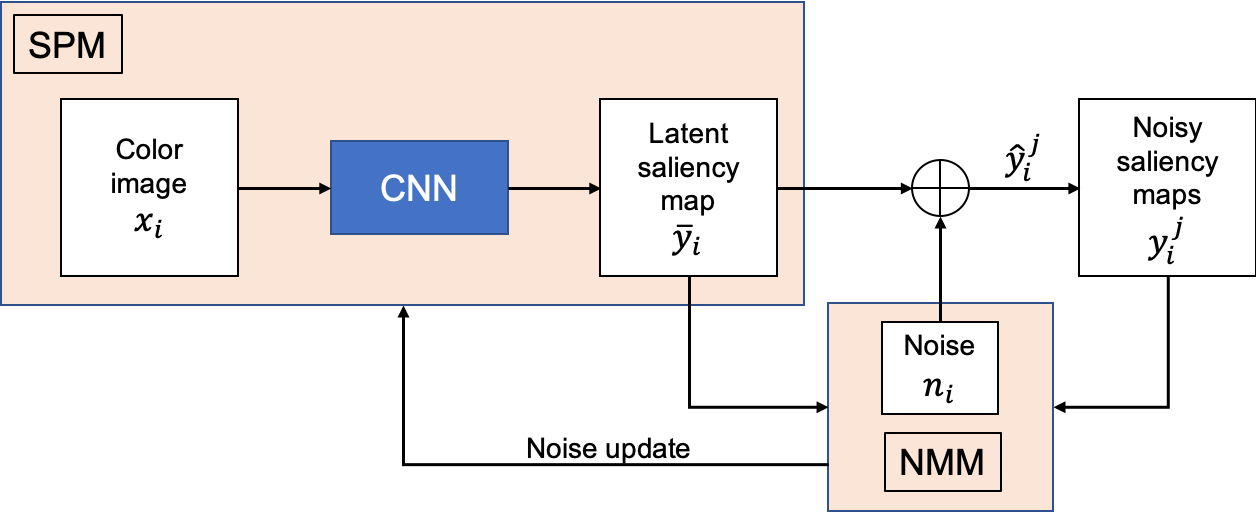
\includegraphics[width=0.4\linewidth]{fig1.png}
  \caption{Schematic representation of the deep unsupervised detection framework.}
  \label{fig:scheme}
\end{figure}

In our project, we propose to reproduce the work of \cite{zhang2018} with MSRA-B dataset \cite{wang2017}, 5000 images with pixel-accurate object labeling, which most  images only have one salient object. Further, the deep unsupervised detection framework (Fig. \ref{fig:scheme}) consists of two connected modules: a saliency prediction model (SPM) that maps from a color image to a latent saliency map with a noise estimation, and a noise modelling module (NMM)  that learns an adaptive noise in noisy saliency maps and updates the noise estimation with the saliency prediction and the noisy salient maps. Both modules works collaboratively with a joint optimization of their parameters. 


\printbibliography

\end{document}